
\documentclass{exam}

\usepackage{graphicx}
\usepackage[fleqn]{amsmath}
\usepackage{unitsdef} 
\usepackage{cancel}
\usepackage{float}
\usepackage{mdwlist}
\usepackage{booktabs}
\usepackage{cancel}
\usepackage{polynom}
\usepackage{caption}
\usepackage{fullpage}
\usepackage{enumerate}

% \newcommand{\degree}{\ensuremath{^\circ}} 
\everymath{\displaystyle}

\newunit{\inch}{in}
\newunit{\foot}{ft}
\newunit{\cemtimeter}{cm}

% \begin{figure}[H]
%   \centering
%   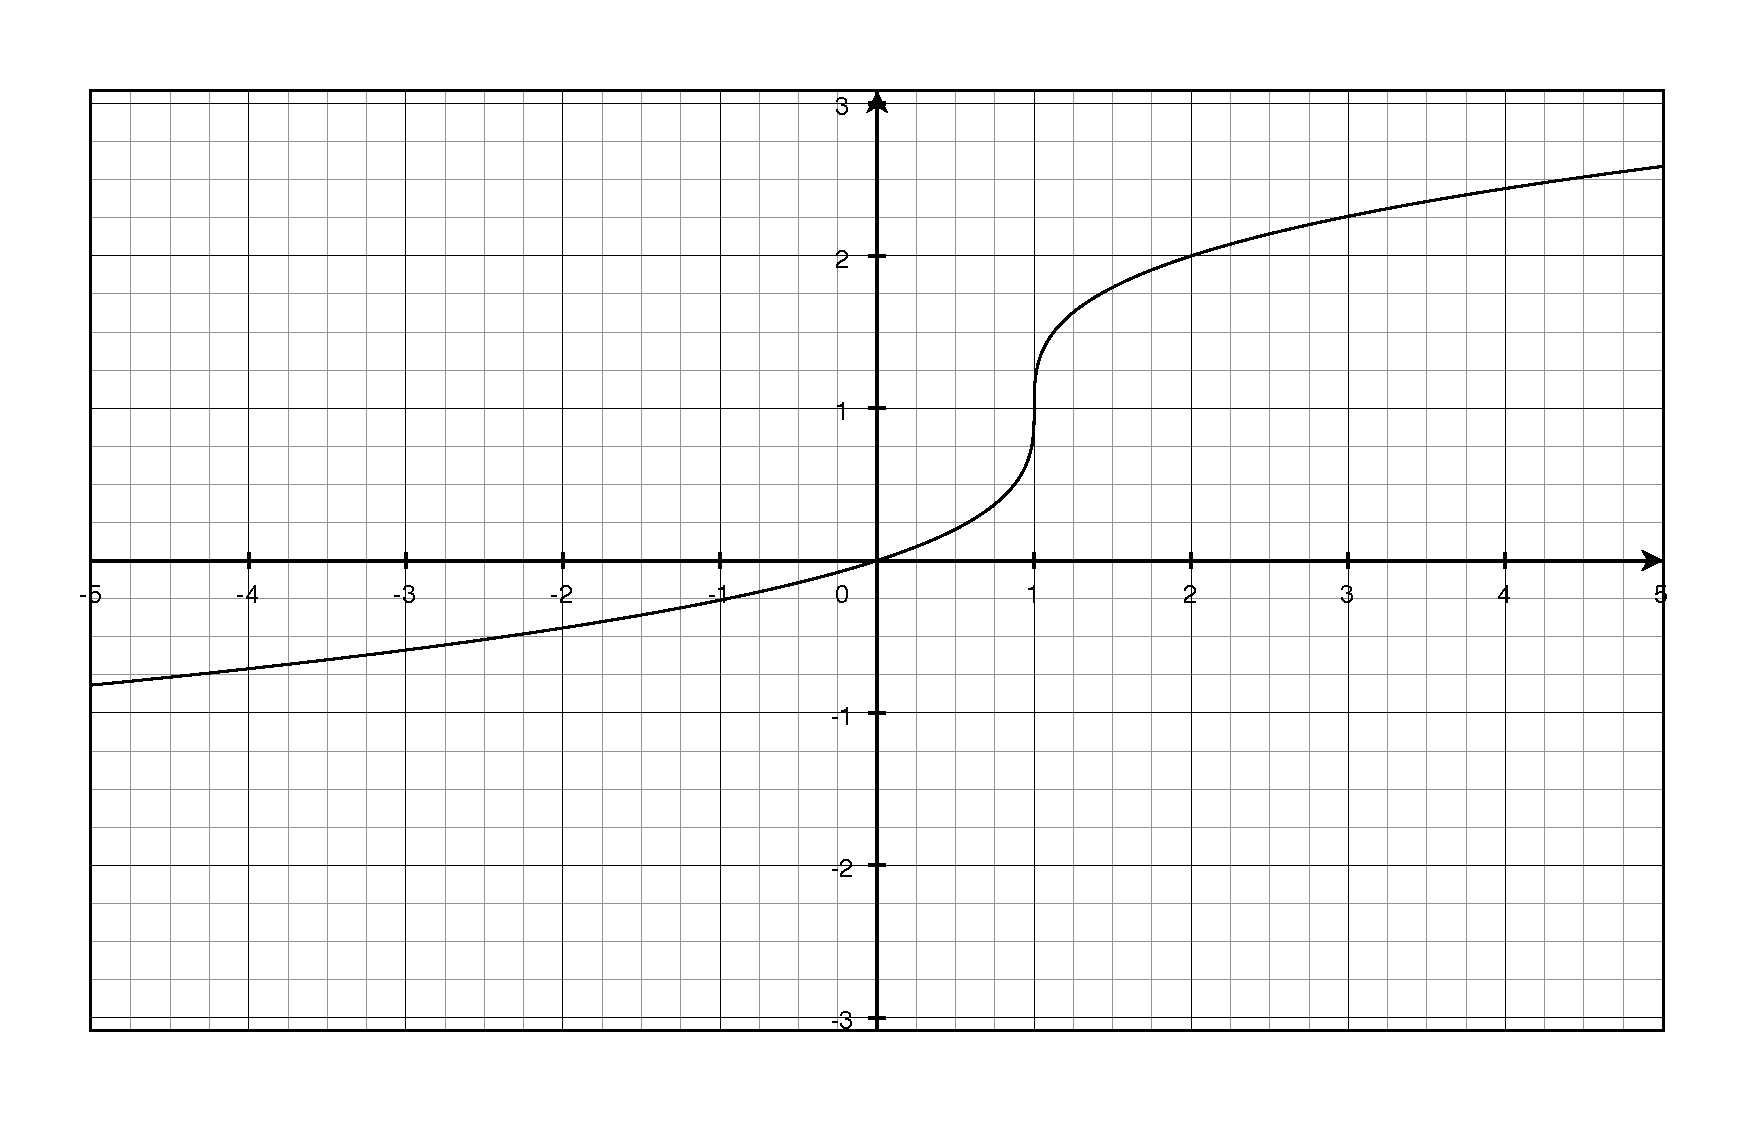
\includegraphics[scale=.3]{question7.eps}
%   \caption*{Question 7}
% \end{figure}

% \begin{tabular}{cc}
% \toprule
% period & amplitude \\
% \midrule
%   $\pi$ & $2$ \\
% \bottomrule
% \end{tabular}

\printanswers

\ifprintanswers 
\usepackage{2in1, lscape} 
\fi

\title{Math 263B \\ Homework Three}
\date{July 26, 2012}

\begin{document}

\maketitle

\section{Homework}

\begin{itemize*}
  \item Read Section 5.3 and 5.4
  \item pp 252-253: 1-2, 4, 7, 9-27, 31-32
  \item pp 260-261: 11-12
\end{itemize*}

\section{Extra Credit}
page 253, problem 45

\ifprintanswers
\pagebreak
\fi

\begin{solution}

Expand the original expression:
\begin{align*}
  \sum_{i = 1}^n &(a_i - a_{i - 1}) b_{i - 1} \\
  &= (a_1 b_0 - a_0 b_0) + (a_2 b_1 - a_1 b_1) + \ldots + (a_n b_{n-1} - a_{n-1} b_{n - 1}) \\
\end{align*}

Rearrange and re-paranenthisize:
\[
  - a_0 b_0 + ( a_1 b_0 - a_1 b_1 ) + (a_2 b_1 - a_2 b_0) + \ldots + a_n b_{n-1} 
\]

Add $a_nb_n - a_nb_n$. This is harmless because this is just zero:
\[
  - a_0 b_0 + ( a_1 b_0 - a_1 b_1 ) + (a_2 b_1 - a_2 b_0) + \ldots + a_n b_{n-1} + (a_n b_n - a_n b_n)
\]

Rearrange:
\[
  - a_0 b_0 + ( a_1 b_0 - a_1 b_1 ) + (a_2 b_1 - a_2 b_0) + \ldots + (a_n b_{n-1} - a_n b_n) + a_n b_n
\]

Write the middle part as a new sum:
\[
  - a_0 b_0 + \sum_{i = 1}^n a_i (b_{i - 1} - b_{i}) + a_n b_n
\]

Rearrange:
\[
  a_n b_n - a_0 b_0 - \sum_{i = 1}^n a_i (b_i - b_{i - 1})
\]

\end{solution}

\ifprintanswers
\pagebreak

\section{Section 5.3}

\begin{description}
\item[1]
\[
  \sum_{k = 1}^6 (k - 1) = 0 + 1 + 2 + 3 + 4 + 5 = 15
\]

\item[2]
\[
  \sum_{i = 1}^6 i^2 = 1 + 4 + 9 + 16 + 25 + 36 = 91
\]

\item[4]
\[
  \sum_{i = 3}^8 (i + 1)^2 = 16 + 25 + 36 + 49 + 64 + 81 = 271
\]

\item[7]
\[
  \sum_{n = 1}^6 n \cos(n \pi) = -1 + 2 - 3 + 4 - 5 + 6 = 3
\]

\item[9]
\[
  \sum_{i = 1}^{41} i
\]

\item[10]
\[
  \sum_{i = 1}^{25} 2i
\]

\item[11]
\[
  \sum_{i = 1}^{100} \frac{1}{i}
\]

\item[12]
\[
  \sum_{i = 1}^{100} \frac{(-1)^{i + 1}}{i}
\]

\item[13]
\[
  \sum_{i = 1}^{50} a_{2i - 1}
\]

\item[14]
\[
  \sum_{i = 0}^{501} b_{2i - 1}
\]

\item[15]
\[
  \sum_{i = 1}^{n} f(c_i)
\]

\item[16]
\[
  \sum_{i = 1}^{n} f(w_i) \Delta x
\]

\item[17]
\[
  \sum_{i = 1}^{10} (a_i + b_i) = \sum_{i = 1}^{10} a_i + \sum_{i = 1}^{10} b_i = 40 + 50 = 90 
\]

\item[18]
\[
  \sum_{i = 1}^{10} (3a_n + 2b_n) = 3 \sum_{i = n}^{10} a_n + 2 \sum_{i = n}^{10} b_n = 120 + 100 = 220
\]

\item[19]
\begin{align*}
  \sum_{p = 0}^{9} (a_{p+1} - b_{p+1}) &= \sum_{p = 1}^{10} (a_i - b_i) \\
  &= \sum_{p = 1}^{10} a_i - \sum_{p = 1}^{10} b_i \\
  &= 40 - 50  \\
  &= -10 \\
\end{align*}

\item[20]
\begin{align*}
  \sum_{q = 1}^{10} (a_q - b_q  - q) &= \sum_{q = 1}^{10} a_q - \sum_{q = 1}^{10} b_q - \sum_{q = 1}^{10} q \\
  &= 40 - 50 - \frac{10 \cdot 11}{2} \\
  &= -65 \\
\end{align*}

\item[21]
\begin{align*}
  \sum_{k = 1}^{40} \left( \frac{1}{k} - \frac{1}{k+1} \right) &= - \sum_{k = 1}^{40} \left(\frac{1}{k+1} -  \frac{1}{k} \right) \\
  &= -(\frac{1}{41} - 1) \\
  &=  1 - \frac{1}{41} \\
  &= \frac{40}{41} \\
\end{align*}

\item[22]
\[
  \sum_{k = 1}^{10} \left( 2^k - 2^{k-1} \right) = 2^{10} - 1 = 1,023
\]

\item[23]
\begin{align*}
  \sum_{k = 3}^{20} \left( \frac{1}{(k+1)^2} - \frac{1}{k^2} \right) &= \frac{1}{21^2} - \frac{1}{3^2} \\
  &= \frac{1}{441} - \frac{1}{9} \\
%  &= \frac{1}{441} - \frac{49}{441} \\
  &= - \frac{48}{441} \\
\end{align*}

  


\item[24]
\[
  \sum_{k = 3}^{m+1} ( a_k - a_{k-1}) = a_{m+1} - a_2
\]

\item[25]
\[
  \sum_{i = 1}^{100} (3i - 2) = 3 \sum_{i = 1}^{100} i - \sum_{i = 1}^{100} 2 = \frac{3 \cdot 100 \cdot 101}{2} - 200 = 14,950
\]

\item[26]
\begin{align*}
  \sum_{i = 1}^{10} [ (i - 1) (4i + 3) ] &= \sum_{i = 1}^{10} 4i^2 - i - 3 \\
  & = \frac{4 \cdot 10 \cdot 11 \cdot 21}{6} - \frac{10 \cdot 11}{2} - 30 \\
  &= 1,455
\end{align*}

\item[27]
\begin{align*}
  \sum_{k = 1}^{10} (k^3 - k^2) &= \left( \frac{10 \cdot 11}{2} \right)^2 - \frac{10 \cdot 11 \cdot 21}{6} \\
  &= 2,640 \\
\end{align*}

\item[31]
\[
  \sum_{k = 1}^{17} k (k + 1)
\]

\item[32]
\[
  \sum_{k = 1}^{10} (k + 4) 2^k
\]

\end{description}

\pagebreak

\section{Section 5.4}

\begin{description}

\item[11]
\begin{align*}
  \sum_{i = 1}^n \left( \frac{i}{n} + 2 \right) \cdot \frac{1}{n} &= \frac{1}{n^2} \sum_{i = 1}^n i + \frac{1}{n} \sum_{i = 1}^n 2 \\
  &= \frac{1}{n^2} \cdot \frac{n(n+1)}{2} + \frac{1}{n} \cdot 2n \\
  &= \frac{5}{2} + \frac{1}{2n} \\
\\
  \lim_{n \to \infty} \left( \frac{5}{2} + \frac{1}{2n} \right) &= \frac{5}{2} \\
\end{align*}

\item[12]
\begin{align*}
  \sum_{i = 1}^n \left[ \frac{1}{2} \cdot \left( \frac{i}{n} \right)^2 + 1 \right] \cdot \frac{1}{n} &= \frac{1}{2n^3} \sum_{i = 1}^n i^2 + \frac{1}{n} \sum_{i = 1}^n 1 \\
  &= \frac{1}{2n^3} \cdot \frac{n(n + 1)(2n +1)}{6} + \frac{1}{n} \cdot n \\ 
  &= \frac{7}{6} + \frac{1}{4n} + \frac{1}{12n^2} \\
\\
  \lim_{n \to \infty} \left( \frac{7}{6} + \frac{1}{4n} + \frac{1}{12n^2} \right) &= \frac{7}{6} \\
\end{align*}


\end{description}

\else

\vspace{10 cm}

%% {\em Some writers have so confounded society with government, as to leave little or no distinction between them; whereas
%%   they are not only different, but have different origins. Society is produced by our wants, and government by our
%%   wickedness; the former promotes our happiness POSITIVELY by uniting our affections, the latter NEGATIVELY by
%%   restraining our vices. The one encourages intercourse, the other creates distinctions. The first a patron, the last a
%%   punisher.}

{\em A long habit of not thinking a thing wrong, gives it a superficial appearance of being right, and raises at first a
  formidable outcry in defense of custom.}

\vspace{.2 cm}

\hspace{1 cm} --Thomas Paine

\fi

\end{document}

